\documentclass{article}
\usepackage[utf8]{inputenc}
\usepackage{graphicx} 

\begin{document}


Voditelj natjecanja započinje proces kreiranja natjecanja slanjem zahtjeva web-aplikaciji.
Web-aplikacija provjerava korisničke role u bazi podataka kako bi utvrdila je li korisnik ovlašten za kreiranje natjecanja.

\textbf{Ako je korisnik voditelj natjecanja:}
\begin{itemize}
  \item Web-aplikacija otvara formu za izradu natjecanja.
  \item Voditelj šalje zahtjev za popis dostupnih zadataka.
  \item Web-aplikacija dohvaća dostupne zadatke iz baze podataka i prikazuje ih voditelju.
  \item Voditelj odabire željene zadatke i kreira natjecanje.
  \item Web-aplikacija sprema informacije o natjecanju u bazu podataka.
  \item Web-aplikacija šalje povratnu informaciju voditelju o uspješnom kreiranju natjecanja.
\end{itemize}

\textbf{Ako korisnik nije voditelj natjecanja:}
\begin{itemize}
  \item Web-aplikacija šalje odgovor voditelju da samo voditelji natjecanja mogu kreirati zadatke.
\end{itemize}


\begin{figure}[h!]
  \centering
  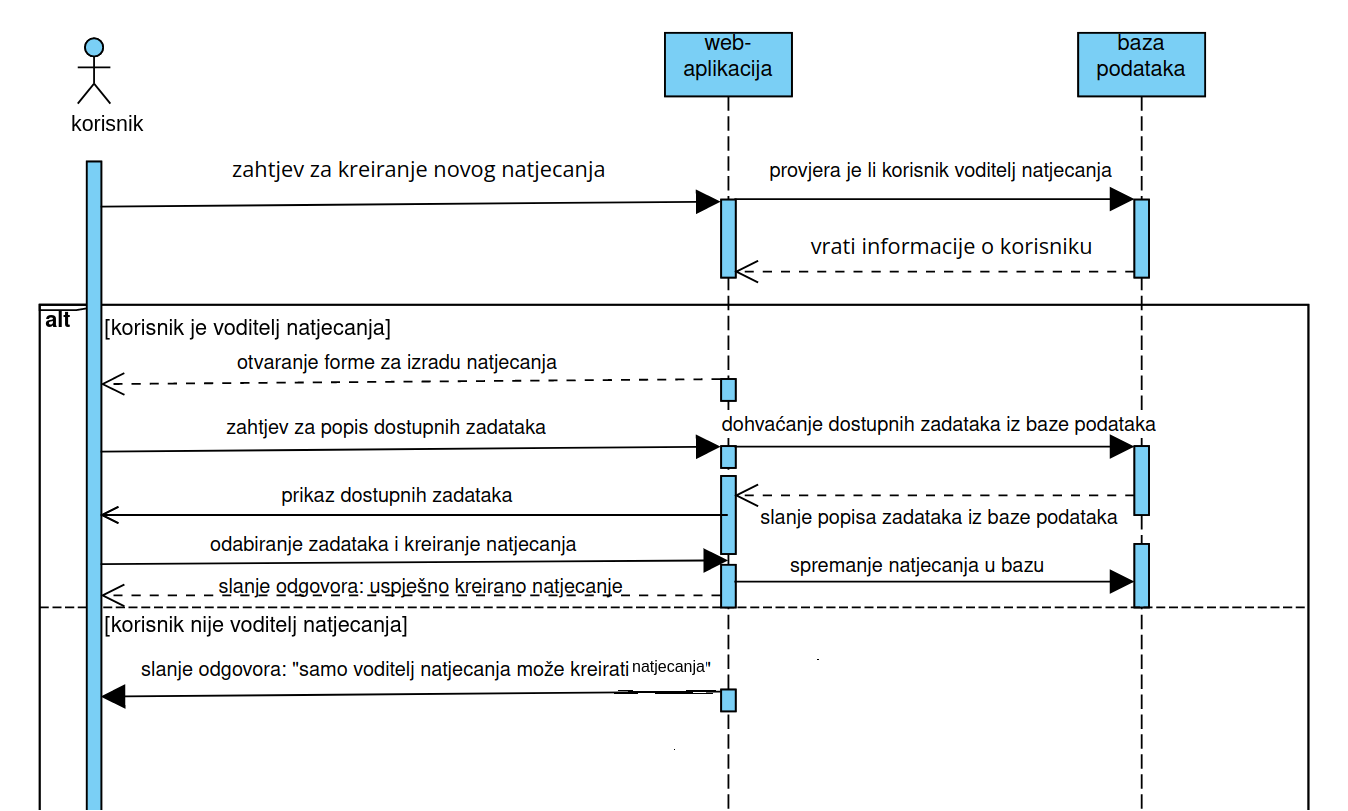
\includegraphics[width=\linewidth]{../slike/kreiranje_natjecanja.png}
  \caption{Sekvencijski dijagram kreiranja novog natjecanja}\label{fig:seqdiag}
\end{figure}

\end{document}
